\documentclass[aspectratio=169,10pt]{beamer}
\usetheme{Madrid}
\usecolortheme{seahorse}

\usepackage[utf8]{inputenc}
\usepackage{amsmath,amssymb,amsthm}
\usepackage{listings}
\usepackage{xcolor}
\usepackage{graphicx}
\usepackage{hyperref}

\graphicspath{{figures/}}

\setbeamertemplate{navigation symbols}{}
\setbeamertemplate{footline}[frame number]

\lstset{
    language=Python,
    basicstyle=\ttfamily\scriptsize,
    keywordstyle=\color{blue},
    commentstyle=\color{green!50!black},
    stringstyle=\color{red},
    showstringspaces=false,
    numbers=left,
    numberstyle=\tiny\color{gray},
    frame=single,
    breaklines=true,
    tabsize=2
}

\title{Inner Product Spaces}
\subtitle{Chapter 1c: Pathak's Introduction to Nonlinear Analysis}
\author{Based on H.K. Pathak (2018)}
\date{2026}

\begin{document}

\frame{\titlepage}

\begin{frame}
\frametitle{Outline}
\tableofcontents[hideallsubsections]
\end{frame}

\section{Section 1.1: Inner Product Spaces - Definitions}

\begin{frame}
\frametitle{Inner Product}

\begin{definition}[Inner Product]
Let $X$ be a complex linear space. A function $\langle \cdot, \cdot \rangle: X \times X \to \mathbb{C}$ is called an \emph{inner product} if for all $x, y, z \in X$ and $\lambda \in \mathbb{C}$:
\begin{itemize}
\item[\textbf{IP1}] $\langle x, x \rangle \geq 0$ (positivity)
\item[\textbf{IP2}] $\langle x, x \rangle = 0 \iff x = 0$ (definiteness)
\item[\textbf{IP3}] $\langle x, y \rangle = \overline{\langle y, x \rangle}$ (conjugate symmetry)
\item[\textbf{IP4}] $\langle \lambda x + y, z \rangle = \lambda \langle x, z \rangle + \langle y, z \rangle$ (linearity in first argument)
\end{itemize}
\end{definition}

\vspace{0.2cm}

An \emph{inner product space} is a linear space with an inner product.

\vspace{0.3cm}

\textbf{Consequences of the definition:}
\begin{itemize}
\item $\langle x, y + z \rangle = \langle x, y \rangle + \langle x, z \rangle$
\item $\langle x, \lambda y \rangle = \overline{\lambda} \langle x, y \rangle$
\end{itemize}
\end{frame}

\begin{frame}
\frametitle{Induced Norm and Cauchy-Schwarz}

\begin{theorem}[Norm Induced by Inner Product]
For any inner product space, the function $\|\cdot\|: X \to \mathbb{R}_+$ defined by
$$\|x\| = \sqrt{\langle x, x \rangle}$$
is a norm on $X$. This is called the \emph{Hilbertian norm}.
\end{theorem}

\vspace{0.3cm}

\begin{theorem}[Cauchy-Schwarz Inequality]
For all $x, y \in X$,
$$|\langle x, y \rangle| \leq \|x\| \cdot \|y\|$$
with equality if and only if $x$ and $y$ are linearly dependent.
\end{theorem}

\vspace{0.3cm}

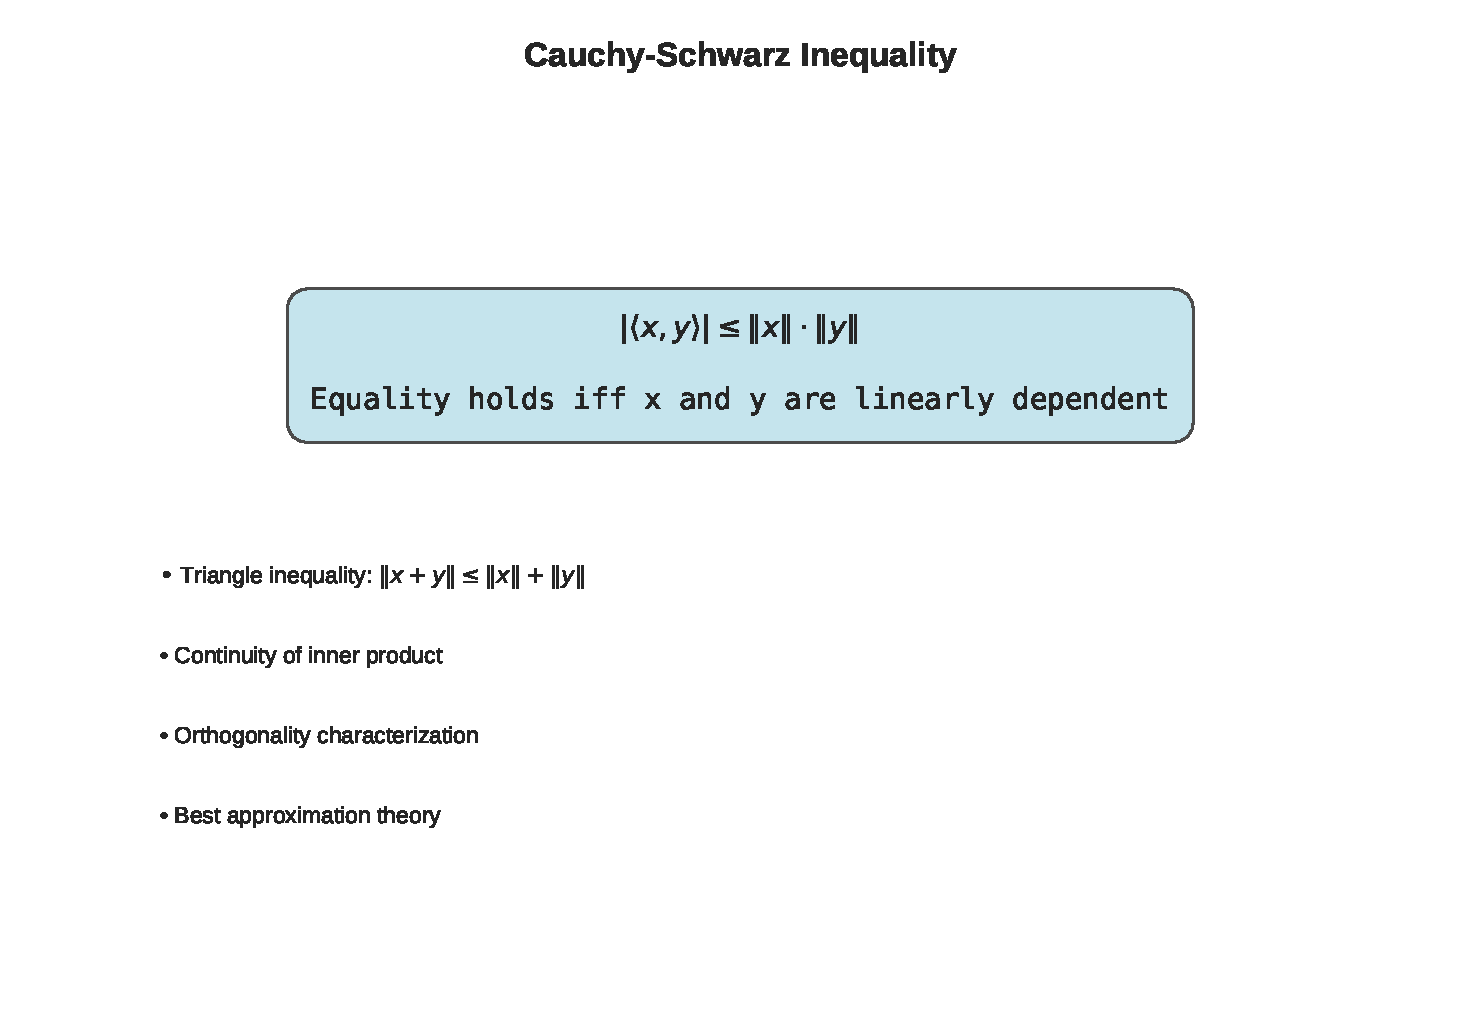
\includegraphics[width=0.8\textwidth]{fig_cauchy_schwarz.pdf}
\end{frame}

\begin{frame}
\frametitle{Parallelogram Law}

\begin{theorem}[Parallelogram Law]
For all $x, y$ in an inner product space:
$$2(\|x\|^2 + \|y\|^2) = \|x+y\|^2 + \|x-y\|^2$$
\end{theorem}

\vspace{0.3cm}

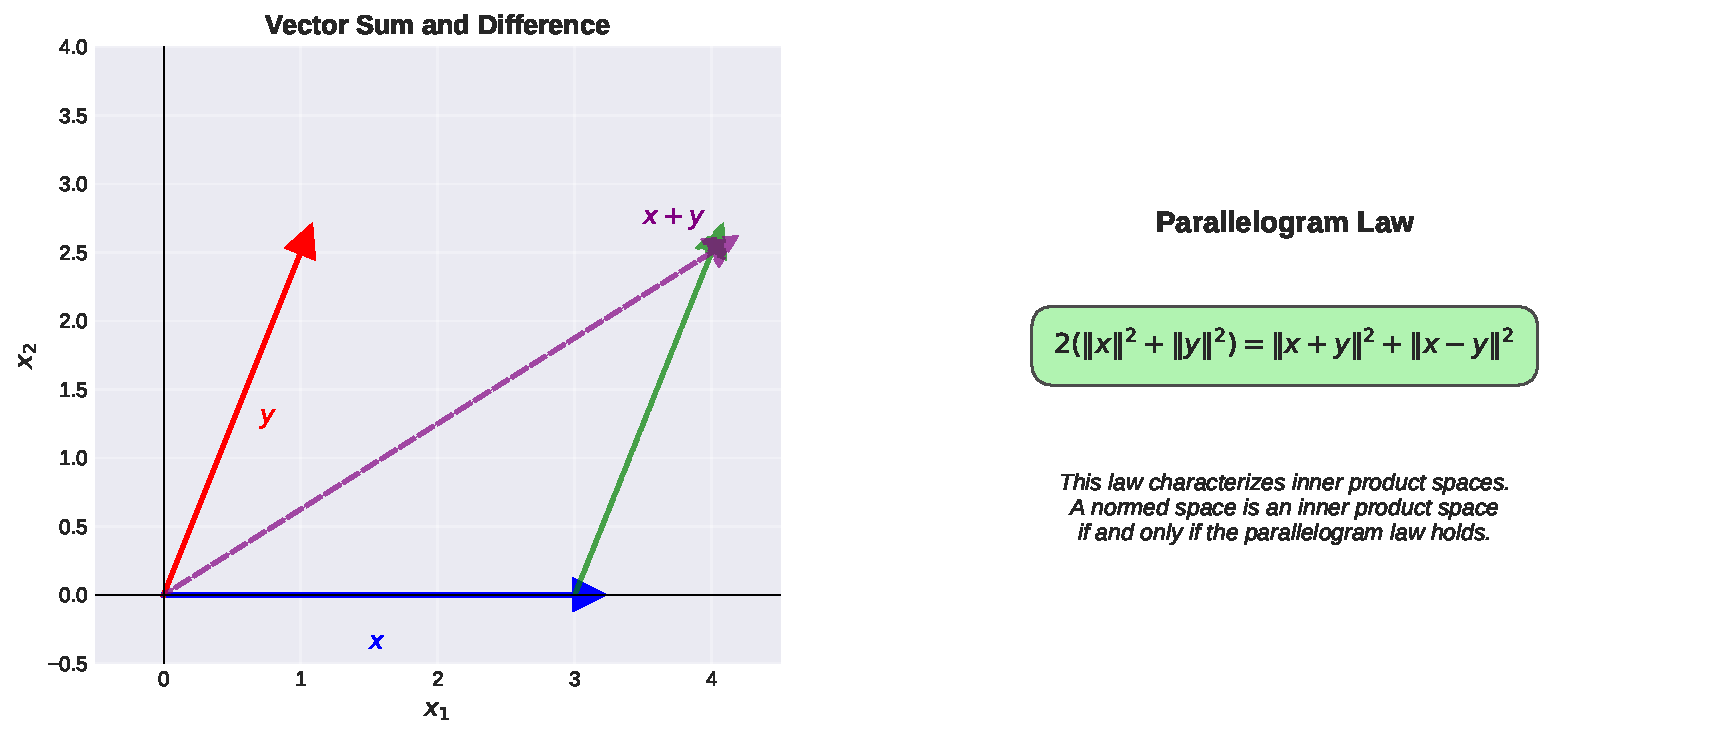
\includegraphics[width=\textwidth]{fig_parallelogram_law.pdf}

\vspace{-0.2cm}

\textbf{Significance:} This characterizes inner product spaces. A normed space is an inner product space if and only if the parallelogram law holds.
\end{frame}

\begin{frame}
\frametitle{Orthogonality}

\begin{definition}[Orthogonal Vectors]
Two vectors $x, y$ in an inner product space are \emph{orthogonal}, denoted $x \perp y$, if
$$\langle x, y \rangle = 0$$
\end{definition}

\vspace{0.3cm}

\begin{theorem}[Pythagorean Theorem]
If $x \perp y$, then
$$\|x + y\|^2 = \|x\|^2 + \|y\|^2$$
\end{theorem}

\vspace{0.3cm}

\begin{definition}[Orthonormal Set]
A set $\{e_i\}_{i \in I}$ is \emph{orthonormal} if:
\begin{itemize}
\item $\langle e_i, e_j \rangle = \delta_{ij}$ (Kronecker delta) for all $i, j \in I$
\item $\delta_{ij} = 1$ if $i = j$, and $\delta_{ij} = 0$ if $i \neq j$
\end{itemize}
\end{definition}

\vspace{0.3cm}

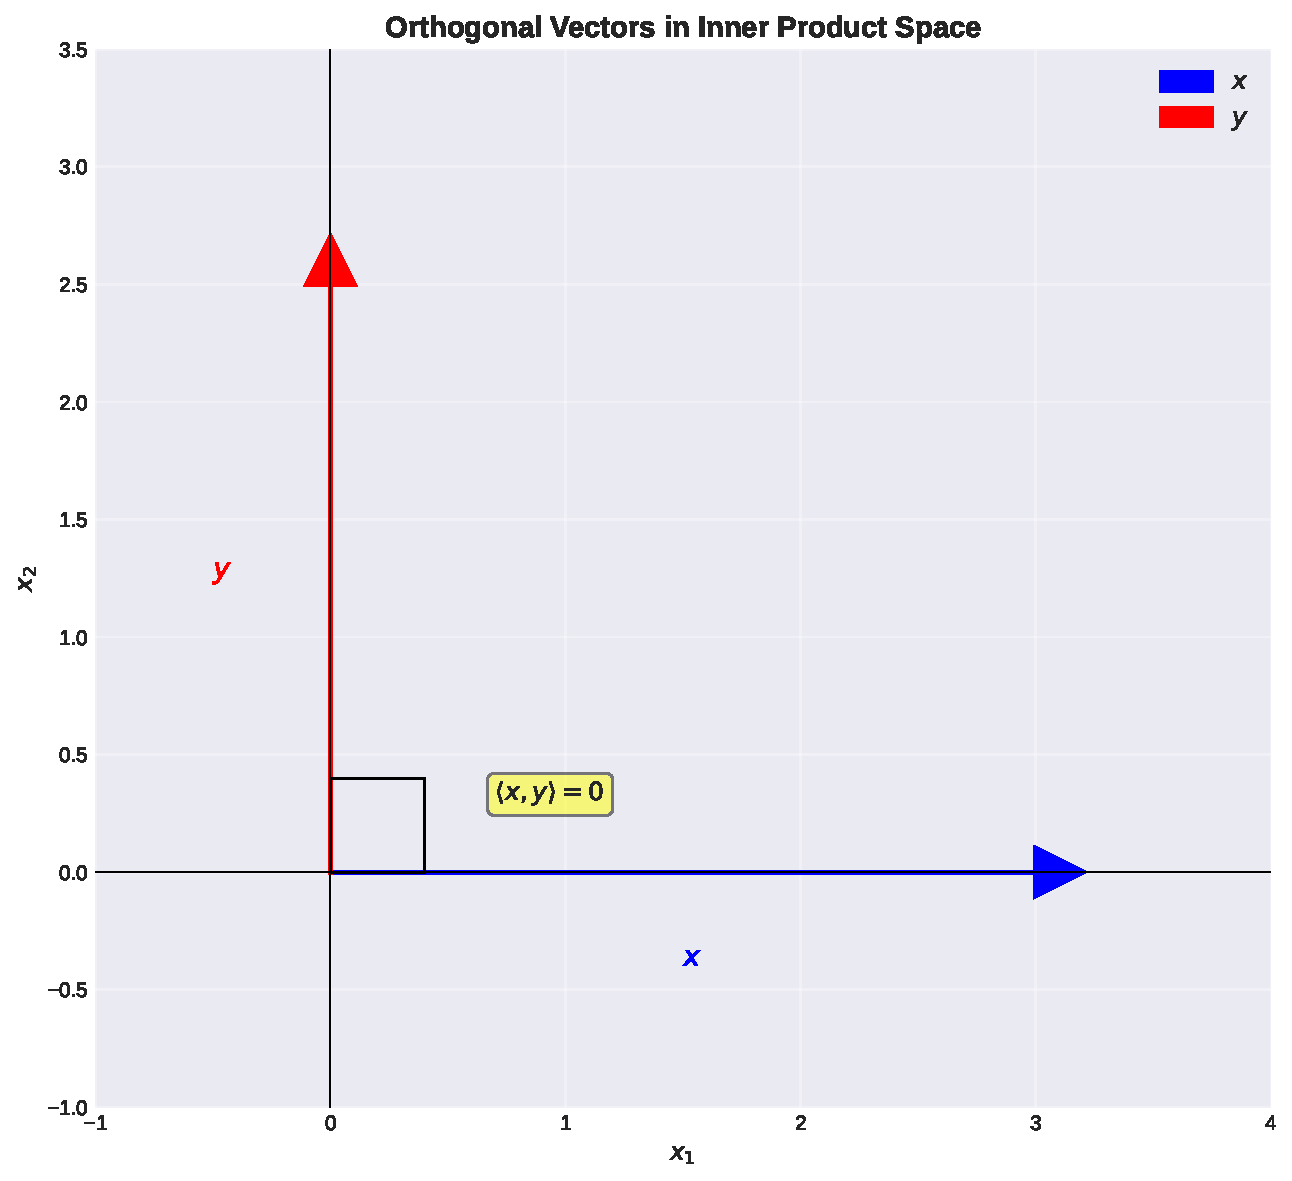
\includegraphics[width=0.7\textwidth]{fig_orthogonality.pdf}
\end{frame}

\section{Section 1.2: Hilbert Spaces}

\begin{frame}
\frametitle{Definition of Hilbert Space}

\begin{definition}[Hilbert Space]
A \emph{Hilbert space} $H$ is a complete inner product space. That is:
\begin{itemize}
\item $H$ is an inner product space with inner product $\langle \cdot, \cdot \rangle$
\item $H$ is complete with respect to the norm $\|x\| = \sqrt{\langle x, x \rangle}$
\item Every Cauchy sequence in $H$ converges to a point in $H$
\end{itemize}
\end{definition}

\vspace{0.3cm}

In other words, a Hilbert space is a complete Banach space with an inner product structure.

\vspace{0.3cm}

\textbf{Remark:}
\begin{itemize}
\item Every Hilbert space is a Banach space
\item Not every Banach space is a Hilbert space (e.g., $\ell^p$ with $p \neq 2$)
\item Hilbert spaces have the special feature of being self-dual
\end{itemize}

\vspace{0.3cm}

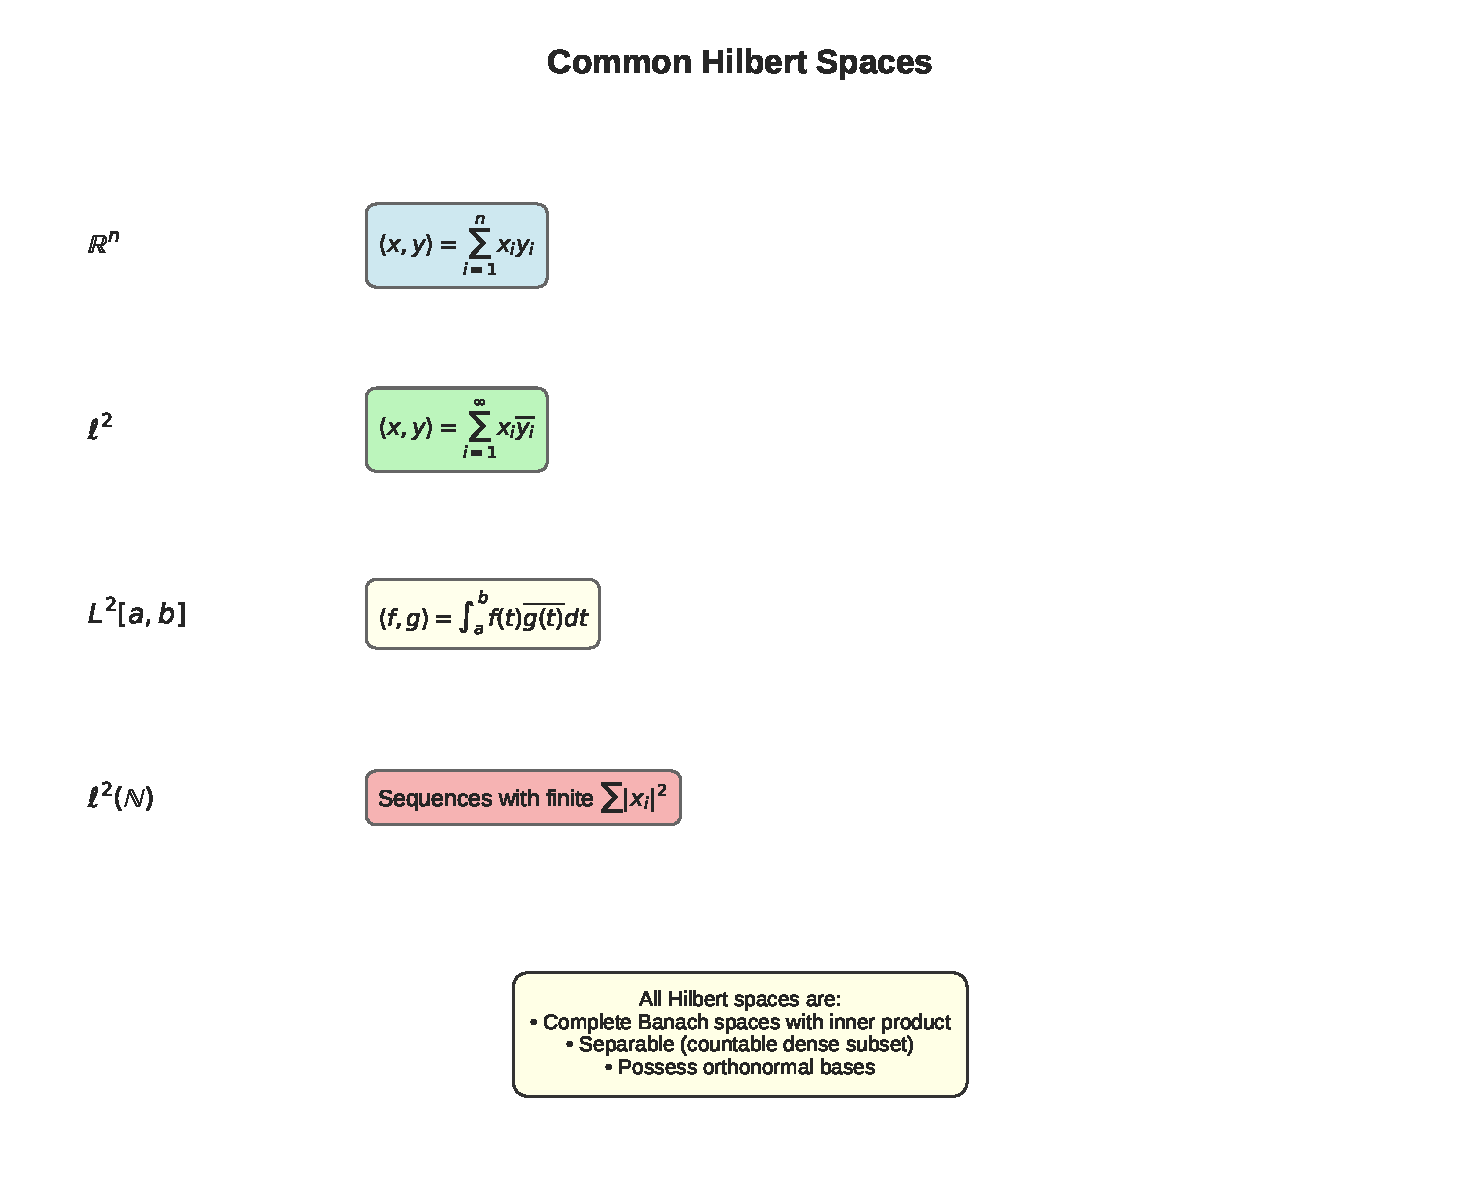
\includegraphics[width=\textwidth]{fig_hilbert_examples.pdf}
\end{frame}

\begin{frame}
\frametitle{Examples of Hilbert Spaces}

\textbf{Example 1: Finite Dimensional}
$$\mathbb{R}^n = \{(x_1, \ldots, x_n) : x_i \in \mathbb{R}\}$$
with $\langle x, y \rangle = \sum_{i=1}^n x_i y_i$, $\|x\|_2 = \sqrt{\sum_{i=1}^n x_i^2}$.

\vspace{0.3cm}

\textbf{Example 2: $\ell^2$ Space}
$$\ell^2 = \left\{ (x_i)_{i=1}^\infty : \sum_{i=1}^\infty |x_i|^2 < \infty \right\}$$
with $\langle x, y \rangle = \sum_{i=1}^\infty x_i \overline{y_i}$ and $\|x\|_2 = \sqrt{\sum_{i=1}^\infty |x_i|^2}$.

\vspace{0.3cm}

\textbf{Example 3: $L^2[a,b]$ Space}
$$L^2[a,b] = \left\{ f: [a,b] \to \mathbb{C} : \int_a^b |f(t)|^2 dt < \infty \right\}$$
with $\langle f, g \rangle = \int_a^b f(t) \overline{g(t)} dt$ and $\|f\| = \sqrt{\int_a^b |f(t)|^2 dt}$.

\vspace{0.3cm}

\textbf{Example 4: Weighted $L^2$ Space}
$$L^2_w[a,b] = \left\{ f : \int_a^b w(t)|f(t)|^2 dt < \infty \right\}$$
where $w(t) > 0$ is a weight function.
\end{frame}

\begin{frame}[fragile]
\frametitle{Numerical Example: The $\ell^2$ Space}

\begin{lstlisting}[language=Python]
import numpy as np

# Example: Geometric series sequence
x = np.array([1/2**i for i in range(1, 20)])
y = np.array([1/3**i for i in range(1, 20)])

# Inner product
inner_prod = np.sum(x * y)
print(f"<x, y> = {inner_prod:.6f}")

# Norms
norm_x = np.linalg.norm(x)
norm_y = np.linalg.norm(y)
print(f"||x|| = {norm_x:.6f}")
print(f"||y|| = {norm_y:.6f}")

# Cauchy-Schwarz check
cs_lhs = abs(inner_prod)
cs_rhs = norm_x * norm_y
print(f"|<x,y>| = {cs_lhs:.6f} <= {cs_rhs:.6f}")
print(f"Inequality satisfied: {cs_lhs <= cs_rhs}")

# Pythagorean theorem: Check orthogonality
z = np.array([(-1)**i / 4**i for i in range(1, 20)])
inner_xz = np.sum(x * z)
norm_x_plus_z = np.linalg.norm(x + z)
norm_x_sq_plus_norm_z_sq = norm_x**2 + np.linalg.norm(z)**2

print(f"\n<x, z> = {inner_xz:.10f} (nearly 0)")
print(f"||x+z||^2 = {norm_x_plus_z**2:.6f}")
print(f"||x||^2 + ||z||^2 = {norm_x_sq_plus_norm_z_sq:.6f}")
\end{lstlisting}
\end{frame}

\section{Section 1.3: Orthogonal Projections}

\begin{frame}
\frametitle{Orthogonal Projection onto Subspaces}

\begin{theorem}[Orthogonal Projection]
Let $M$ be a closed convex subset of a Hilbert space $H$. For each $x \in H$, there exists a unique point $P_M(x) \in M$ (the \emph{projection} of $x$ onto $M$) such that
$$\|x - P_M(x)\| = \min_{y \in M} \|x - y\|$$
Moreover, $P_M(x)$ is characterized by:
$$\langle x - P_M(x), y - P_M(x) \rangle \leq 0 \quad \text{for all } y \in M$$
\end{theorem}

\vspace{0.3cm}


\includegraphics[width=0.8\textwidth]{fig_projection.pdf}

\vspace{0.2cm}

\textbf{For linear subspaces:} $P_M(x)$ satisfies $\langle x - P_M(x), y \rangle = 0$ for all $y \in M$.
\end{frame}

\begin{frame}
\frametitle{Orthogonal Projection - Algebraic Properties}

\begin{theorem}[Projection Operator Properties]
If $M$ is a closed linear subspace of $H$, then:
\begin{itemize}
\item $P_M: H \to M$ is a linear operator
\item $P_M^2 = P_M$ (idempotence): $P_M(P_M(x)) = P_M(x)$
\item $\|P_M(x)\| \leq \|x\|$ for all $x \in H$ (contractivity)
\item $H = M \oplus M^\perp$ (orthogonal decomposition)
\item $P_{M^\perp} = I - P_M$ (complementary projection)
\end{itemize}
\end{theorem}

\vspace{0.3cm}

\begin{definition}[Orthogonal Complement]
The \emph{orthogonal complement} of $M$ is
$$M^\perp = \{x \in H : \langle x, y \rangle = 0 \text{ for all } y \in M\}$$
\end{definition}

\vspace{0.3cm}

\textbf{Application:} Every vector $x \in H$ can be uniquely written as
$$x = P_M(x) + P_{M^\perp}(x)$$
where $P_M(x) \in M$ and $P_{M^\perp}(x) \in M^\perp$.
\end{frame}

\section{Section 1.4: Orthonormal Bases and Fourier Series}

\begin{frame}
\frametitle{Gram-Schmidt Orthogonalization Process}

\begin{theorem}[Gram-Schmidt Process]
Let $\{v_1, v_2, v_3, \ldots\}$ be a linearly independent sequence in an inner product space. Then there exists an orthonormal sequence $\{e_1, e_2, e_3, \ldots\}$ such that for each $n$, the span of $\{e_1, \ldots, e_n\}$ equals the span of $\{v_1, \ldots, v_n\}$.
\end{theorem}

\vspace{0.2cm}

\textbf{Procedure:}

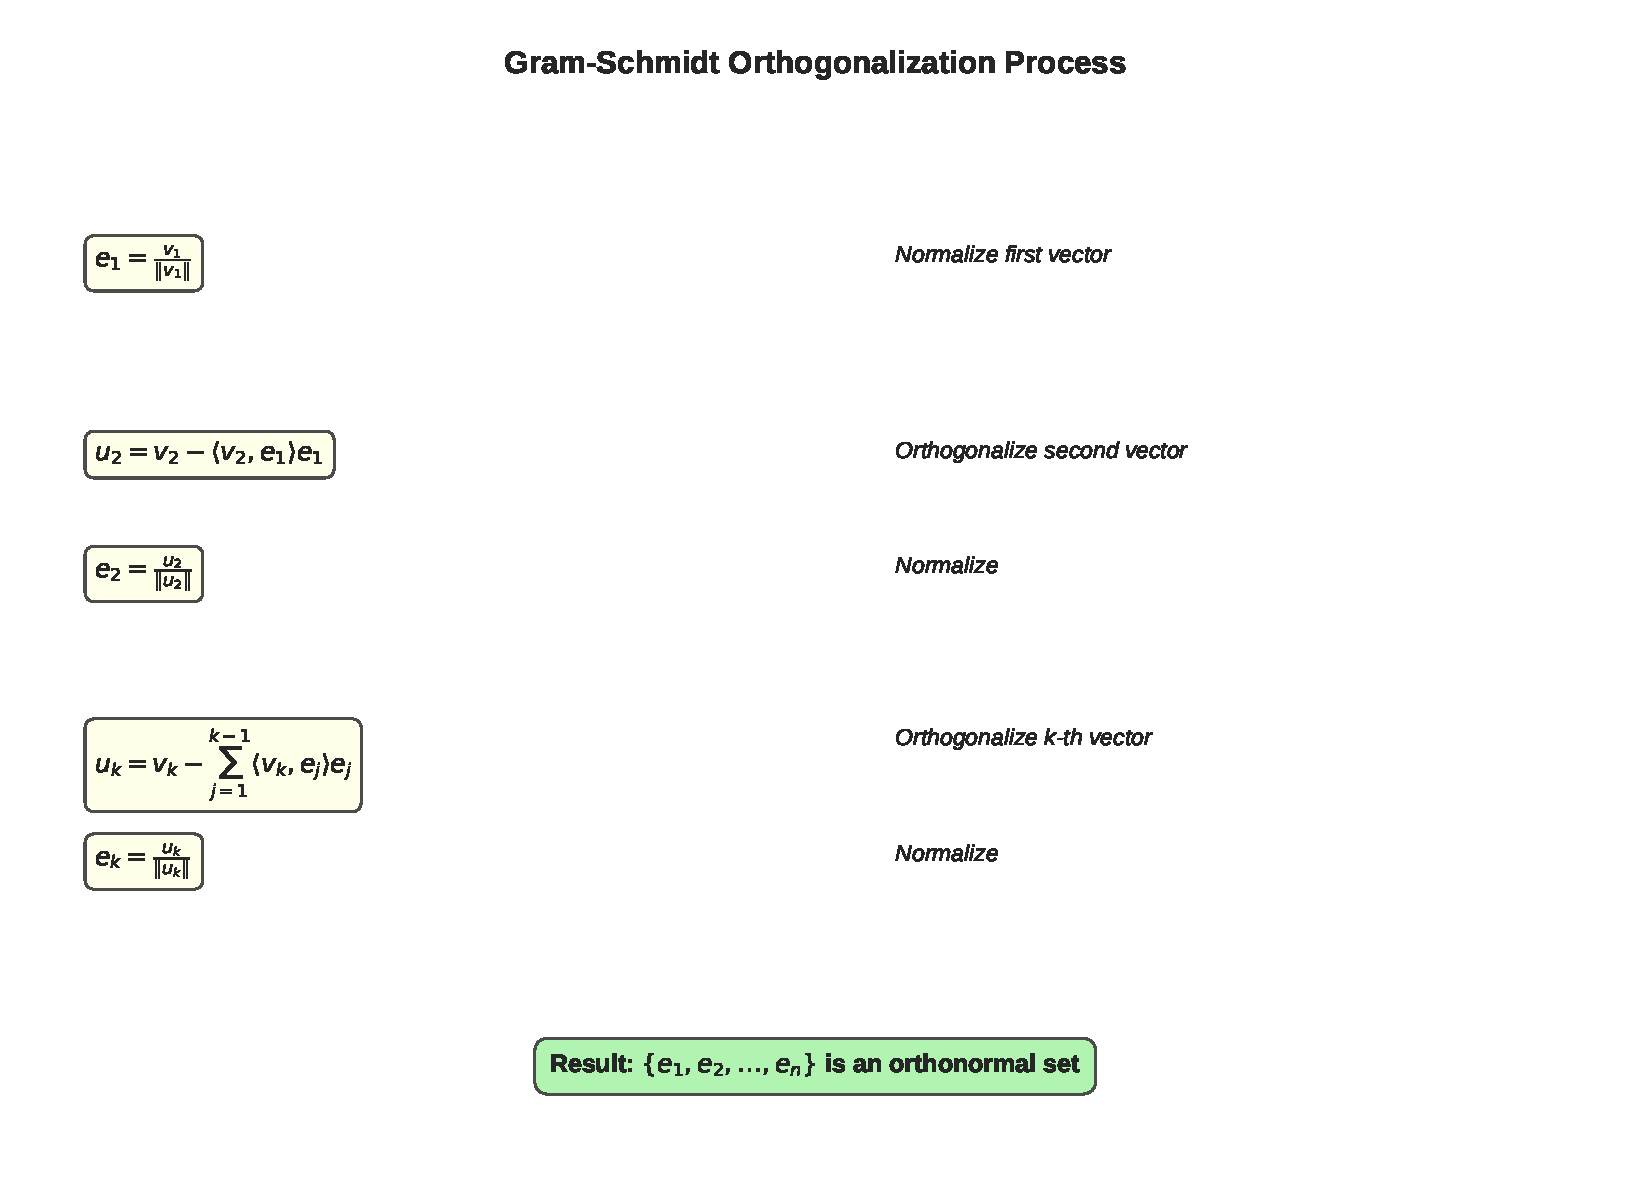
\includegraphics[width=\textwidth]{fig_gram_schmidt.pdf}

\vspace{0.2cm}

\textbf{Consequence:} Every separable inner product space has a countable orthonormal basis.
\end{frame}

\begin{frame}
\frametitle{Complete Orthonormal Systems}

\begin{definition}[Complete Orthonormal System]
A set $\{e_i\}_{i \in I}$ is a \emph{complete orthonormal system} (CONS) if:
\begin{itemize}
\item It is orthonormal: $\langle e_i, e_j \rangle = \delta_{ij}$
\item It is complete: if $\langle x, e_i \rangle = 0$ for all $i \in I$, then $x = 0$
\end{itemize}
\end{definition}

\vspace{0.3cm}

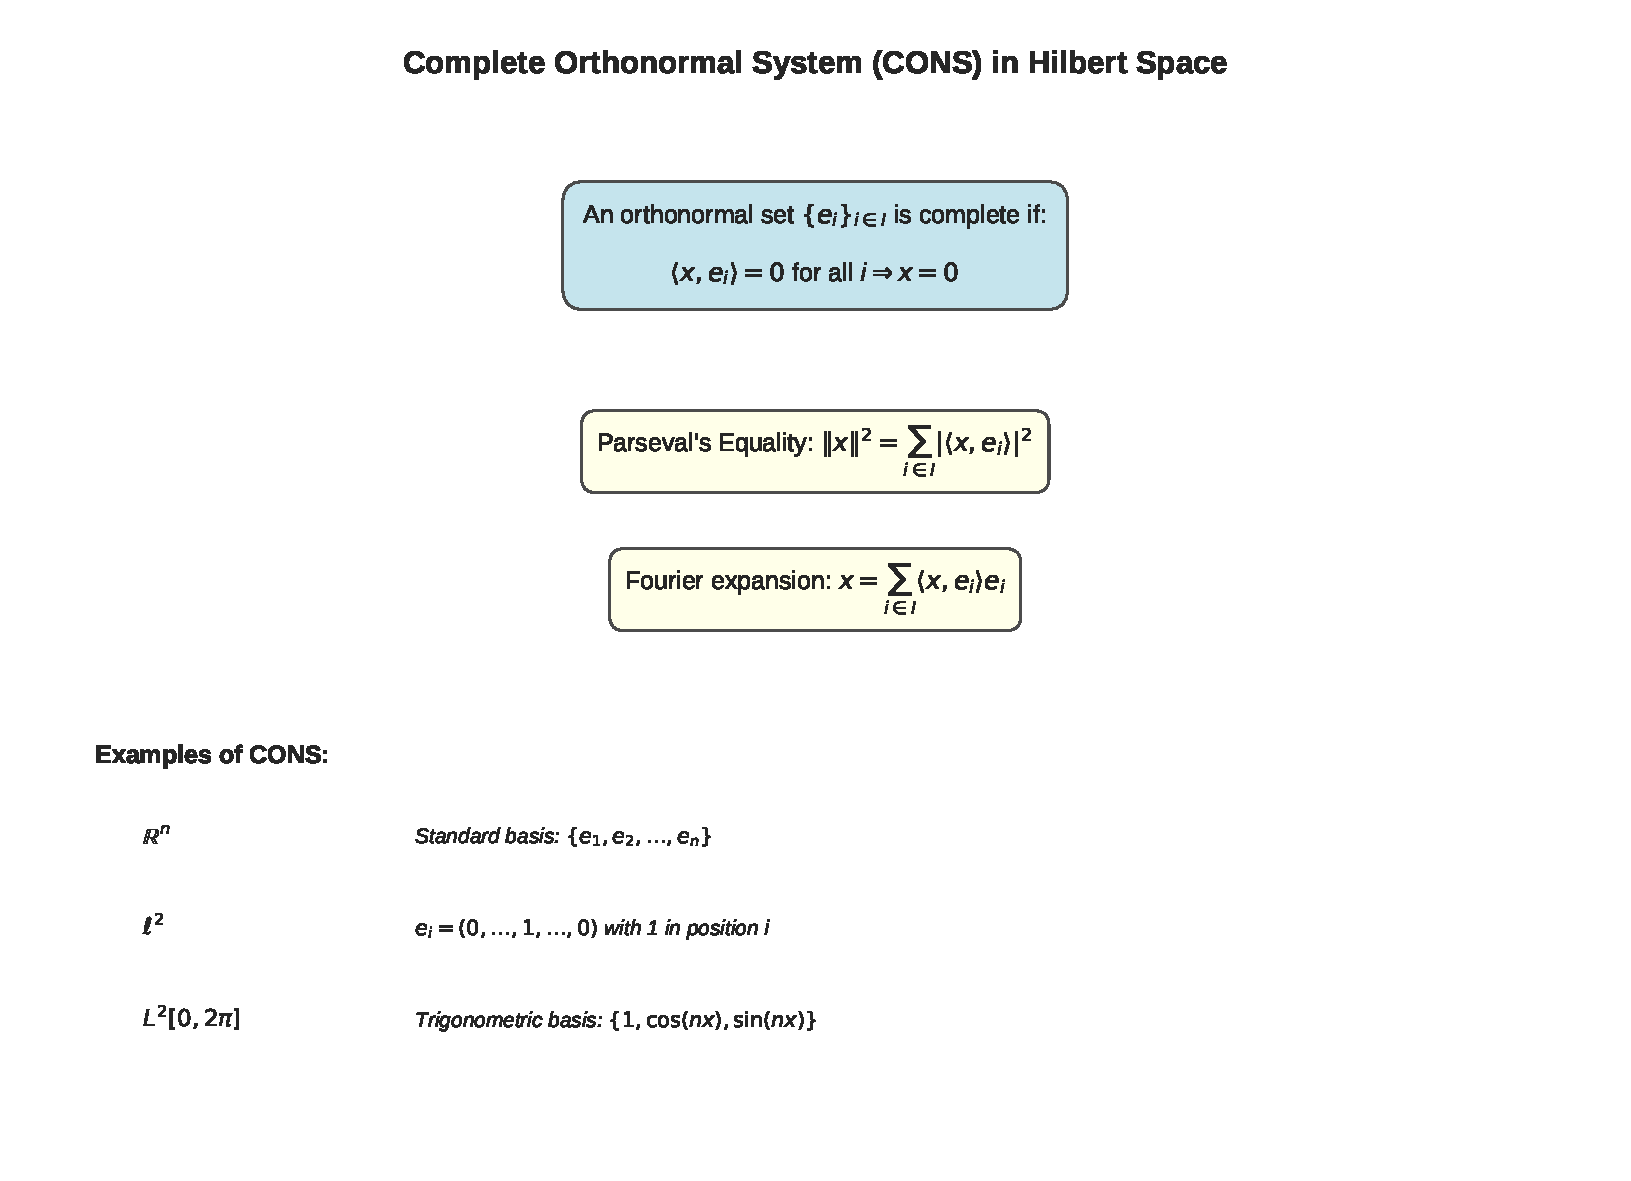
\includegraphics[width=\textwidth]{fig_orthonormal_system.pdf}

\vspace{0.2cm}

\textbf{Key property:} In a separable Hilbert space, every element $x \in H$ can be expanded as
$$x = \sum_{i=1}^\infty c_i e_i \quad \text{where} \quad c_i = \langle x, e_i \rangle$$
This is called the \emph{Fourier expansion} of $x$.
\end{frame}

\begin{frame}
\frametitle{Parseval's Equality}

\begin{theorem}[Parseval's Equality]
Let $\{e_i\}_{i=1}^\infty$ be a complete orthonormal system in a Hilbert space $H$. Then for all $x \in H$:
$$\|x\|^2 = \sum_{i=1}^\infty |\langle x, e_i \rangle|^2$$
\end{theorem}

\vspace{0.3cm}

\textbf{Consequence:} The Fourier coefficients $c_i = \langle x, e_i \rangle$ form an $\ell^2$ sequence.

\vspace{0.3cm}

\begin{example}[Trigonometric Basis in $L^2[0, 2\pi]$]
The orthonormal system
$$\left\{ \frac{1}{\sqrt{2\pi}}, \frac{\cos(nx)}{\sqrt{\pi}}, \frac{\sin(nx)}{\sqrt{\pi}} : n \in \mathbb{N} \right\}$$
is complete in $L^2[0, 2\pi]$, yielding the classical Fourier series.
\end{example}

\vspace{0.3cm}

For $f \in L^2[0, 2\pi]$:
$$\int_0^{2\pi} |f(x)|^2 dx = 2\pi a_0^2 + \pi \sum_{n=1}^\infty (a_n^2 + b_n^2)$$
where $a_n, b_n$ are the Fourier coefficients.
\end{frame}

\section{Section 1.5: Riesz Representation Theorem}

\begin{frame}
\frametitle{Riesz Representation Theorem}

\begin{theorem}[Riesz Representation Theorem]
Let $H$ be a Hilbert space and $f: H \to \mathbb{C}$ a bounded linear functional. Then there exists a unique $y \in H$ such that
$$f(x) = \langle x, y \rangle \quad \text{for all } x \in H$$
Moreover, $\|f\| = \|y\|$.
\end{theorem}

\vspace{0.3cm}

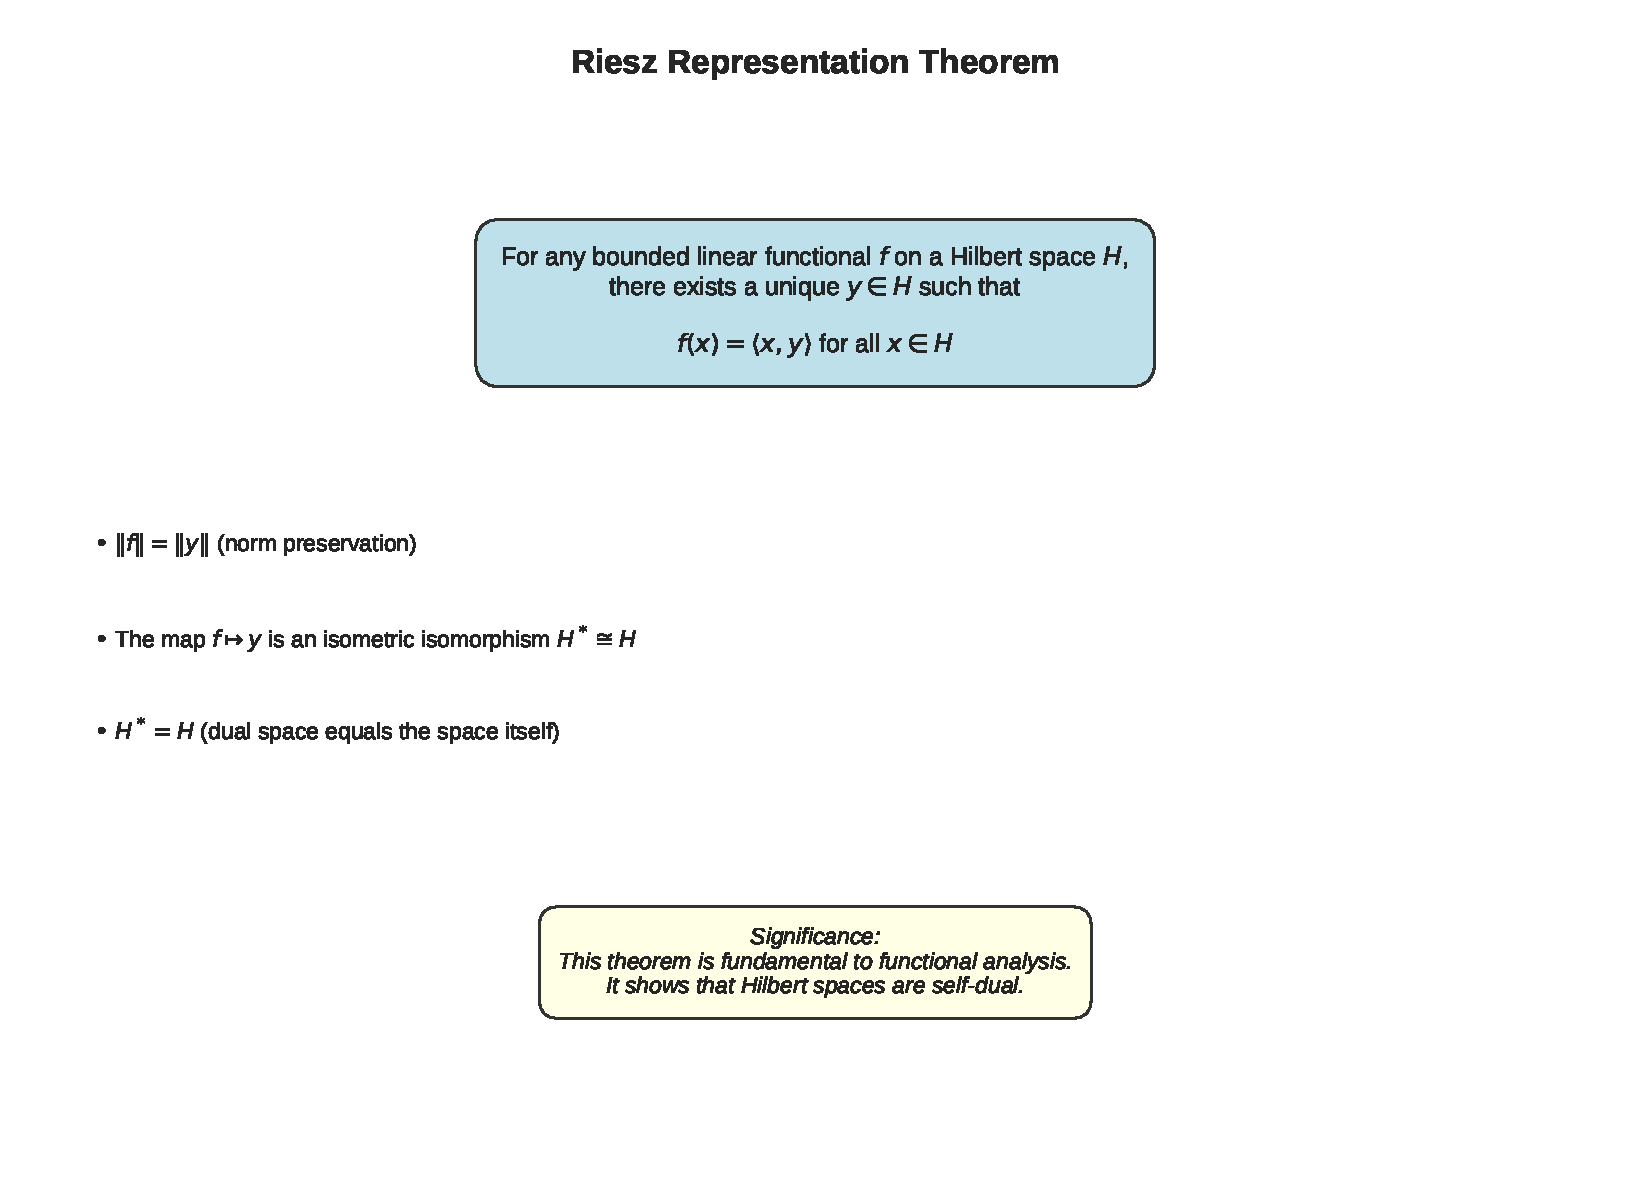
\includegraphics[width=\textwidth]{fig_riesz_theorem.pdf}

\vspace{0.2cm}

\textbf{Consequences:}
\begin{itemize}
\item The dual space $H^* = \{$all bounded linear functionals on $H\}$ is isometrically isomorphic to $H$
\item This is written as $H^* \cong H$ (Hilbert spaces are self-dual)
\item The map $\varphi: H \to H^*$ defined by $\varphi(y)(x) = \langle x, y \rangle$ is a surjective isometry
\end{itemize}
\end{frame}

\begin{frame}
\frametitle{Application: Linear Equations in Hilbert Spaces}

\begin{theorem}[Lax-Milgram Theorem]
Let $a: H \times H \to \mathbb{C}$ be a bounded bilinear form satisfying:
\begin{itemize}
\item Boundedness: $|a(x,y)| \leq M\|x\|\|y\|$ for some $M > 0$
\item Coercivity: $|a(x,x)| \geq m\|x\|^2$ for some $m > 0$
\end{itemize}
Then for each bounded linear functional $f: H \to \mathbb{C}$, there exists a unique $u \in H$ such that
$$a(u, v) = f(v) \quad \text{for all } v \in H$$
\end{theorem}

\vspace{0.3cm}

\textbf{Significance:}
\begin{itemize}
\item Ensures solvability of abstract variational problems
\item Applies to weak formulations of PDEs
\item Fundamental for numerical methods (finite element methods)
\end{itemize}
\end{frame}

\section{Section 1.6: Convergence in Hilbert Spaces}

\begin{frame}
\frametitle{Modes of Convergence}


\includegraphics[width=\textwidth]{fig_convergence.pdf}

\vspace{0.2cm}

\begin{definition}[Strong Convergence]
A sequence $\{x_n\}$ \emph{converges strongly} to $x$, written $x_n \to x$, if $\|x_n - x\| \to 0$.
\end{definition}

\begin{definition}[Weak Convergence]
A sequence $\{x_n\}$ \emph{converges weakly} to $x$, written $x_n \rightharpoonup x$, if
$$\langle x_n, y \rangle \to \langle x, y \rangle \quad \text{for all } y \in H$$
\end{definition}

\vspace{0.3cm}

\textbf{Key difference:} Strong convergence $\Rightarrow$ Weak convergence, but NOT vice versa.
\end{frame}

\begin{frame}
\frametitle{Properties of Weak Convergence}

\begin{theorem}[Properties of Weakly Convergent Sequences]
If $x_n \rightharpoonup x$ in $H$, then:
\begin{itemize}
\item The sequence $\{\|x_n\|\}$ is bounded
\item $\|x\| \leq \liminf_{n \to \infty} \|x_n\|$ (lower semicontinuity of norm)
\item The limit $x$ is unique
\item If $x_n \to x$ strongly, then $x_n \rightharpoonup x$ (strong implies weak)
\end{itemize}
\end{theorem}

\vspace{0.3cm}

\begin{example}[Weak Convergence Without Strong Convergence]
In $\ell^2$, let $e_n$ be the $n$-th standard basis vector. Then:
\begin{itemize}
\item $e_n \rightharpoonup 0$ (weak convergence)
\item $\|e_n - 0\| = 1$ for all $n$ (no strong convergence)
\end{itemize}
\end{example}

\vspace{0.3cm}

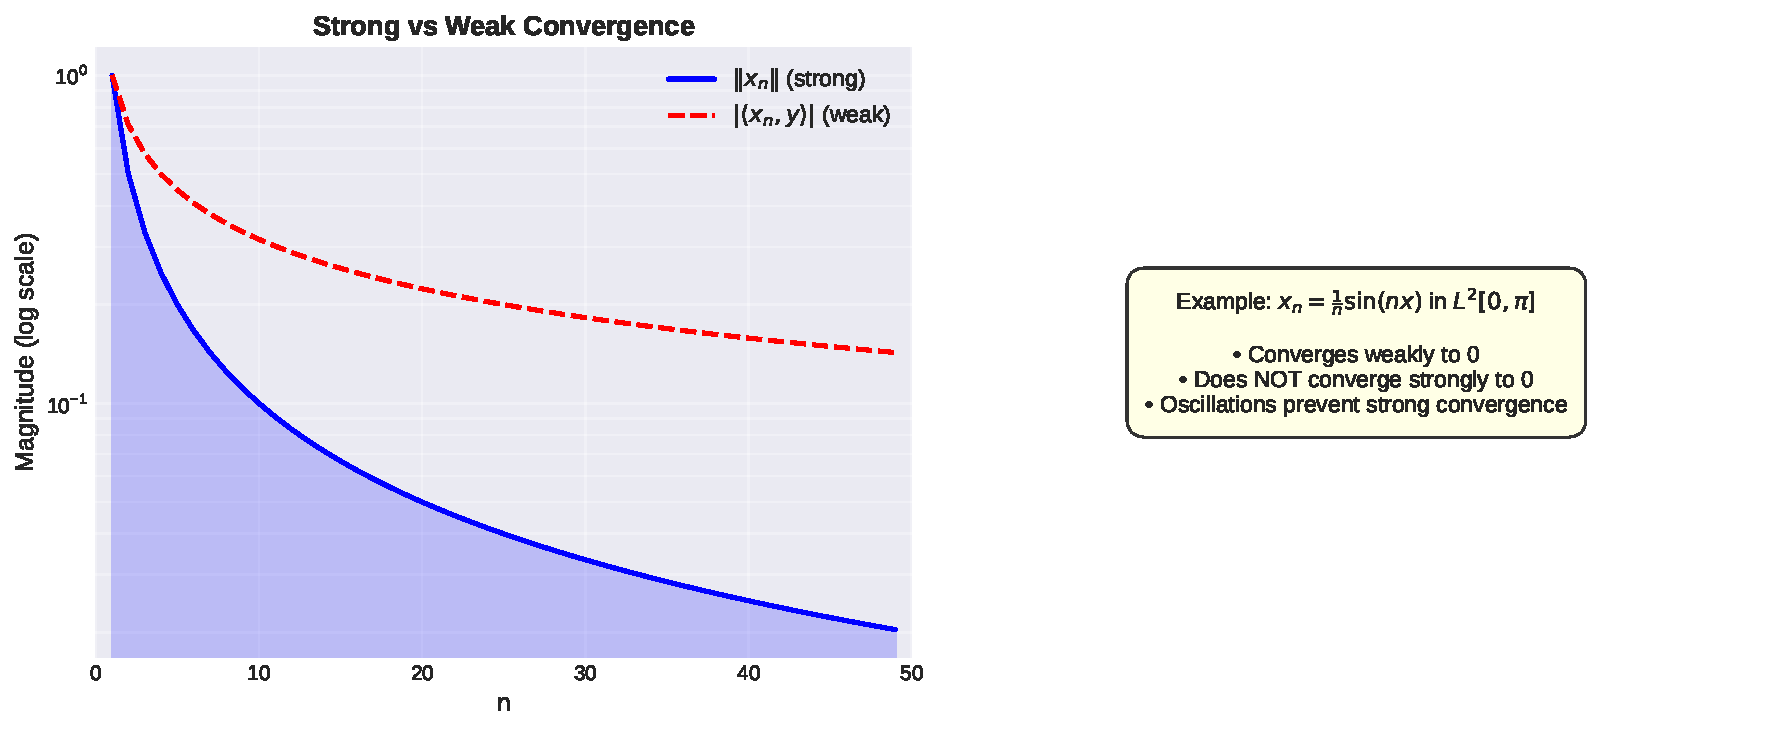
\includegraphics[width=0.8\textwidth]{fig_convergence_example.pdf}
\end{frame}

\begin{frame}
\frametitle{Compactness in Hilbert Spaces}

\begin{theorem}[Eberlein-Smulian Theorem]
A subset $C$ of a Hilbert space $H$ is weakly compact if and only if it is weakly sequentially compact. That is, every sequence in $C$ has a weakly convergent subsequence.
\end{theorem}

\vspace{0.3cm}

\begin{theorem}[Weak Compactness of Closed Balls]
In an infinite-dimensional Hilbert space:
\begin{itemize}
\item Closed balls are weakly compact but NOT compact (in the strong topology)
\item Every bounded sequence has a weakly convergent subsequence
\item This is the basis for many existence results in analysis
\end{itemize}
\end{theorem}

\vspace{0.3cm}

\textbf{Consequence:} Variational problems in Hilbert spaces often have solutions because:
\begin{enumerate}
\item Minimizing sequences are bounded
\item Bounded sequences have weakly convergent subsequences
\item Many functionals are weakly lower semicontinuous
\end{enumerate}
\end{frame}

\section{Section 1.7: Operators in Hilbert Spaces}

\begin{frame}
\frametitle{Linear Operators in Hilbert Spaces}

\begin{definition}[Bounded Linear Operator]
A linear operator $A: H_1 \to H_2$ between Hilbert spaces is \emph{bounded} if
$$\|A\| = \sup_{\|x\|=1} \|Ax\| < \infty$$
\end{definition}

\vspace{0.3cm}

\begin{definition}[Adjoint Operator]
For a bounded linear operator $A: H \to H$, the \emph{adjoint} $A^*: H \to H$ is defined by
$$\langle Ax, y \rangle = \langle x, A^* y \rangle \quad \text{for all } x, y \in H$$
\end{definition}

\vspace{0.3cm}

\textbf{Properties of the adjoint:}
\begin{itemize}
\item $(A^*)^* = A$ (involution)
\item $(A + B)^* = A^* + B^*$
\item $(\lambda A)^* = \overline{\lambda} A^*$
\item $(AB)^* = B^* A^*$ (reverse order)
\item $\|A^*\| = \|A\|$
\end{itemize}
\end{frame}

\begin{frame}
\frametitle{Special Classes of Operators}

\begin{definition}[Self-Adjoint Operator]
An operator $A$ is \emph{self-adjoint} if $A = A^*$, i.e.,
$$\langle Ax, y \rangle = \langle x, Ay \rangle \quad \text{for all } x, y \in H$$
\end{definition}

\begin{definition}[Unitary Operator]
An operator $U$ is \emph{unitary} if $U^* U = U U^* = I$ (isometry and surjective).
\end{definition}

\begin{definition}[Normal Operator]
An operator $A$ is \emph{normal} if $A^* A = A A^*$.
\end{definition}

\begin{definition}[Compact Operator]
An operator $A$ is \emph{compact} if it maps bounded sets to relatively compact sets.
\end{definition}

\vspace{0.3cm}

\textbf{Spectral decomposition:} Compact self-adjoint operators have countable spectrum with eigenvectors forming a complete orthonormal basis.
\end{frame}

\begin{frame}[fragile]
\frametitle{Numerical Example: Operators in $\ell^2$}

\begin{lstlisting}[language=Python]
import numpy as np

# Define an orthonormal basis in R^5 approximating l^2
n = 100
e = np.eye(n)  # Standard basis

# Define a self-adjoint operator: diagonal matrix
lamda = np.array([1 - i/n for i in range(n)])
A = np.diag(lamda)

# Test: <Ax, y> = <x, A*y> = <x, Ay>
x = np.ones(n) / np.sqrt(n)
y = np.zeros(n)
y[:10] = 1/np.sqrt(10)

lhs = np.dot(A @ x, y)
rhs = np.dot(x, A @ y)
print(f"<Ax, y> = {lhs:.6f}")
print(f"<x, Ay> = {rhs:.6f}")
print(f"Self-adjoint test passed: {np.isclose(lhs, rhs)}")

# Compute eigenvalues
eigenvalues = np.diag(A)
print(f"\nEigenvalues (first 10): {eigenvalues[:10]}")
print(f"Operator norm ||A|| = {np.max(np.abs(eigenvalues)):.6f}")

# Check spectrum property
spectrum_radius = np.max(np.abs(eigenvalues))
print(f"Spectral radius = {spectrum_radius:.6f}")
\end{lstlisting}
\end{frame}

\section{Section 1.8: Applications and Summary}

\begin{frame}
\frametitle{Applications of Hilbert Space Theory}

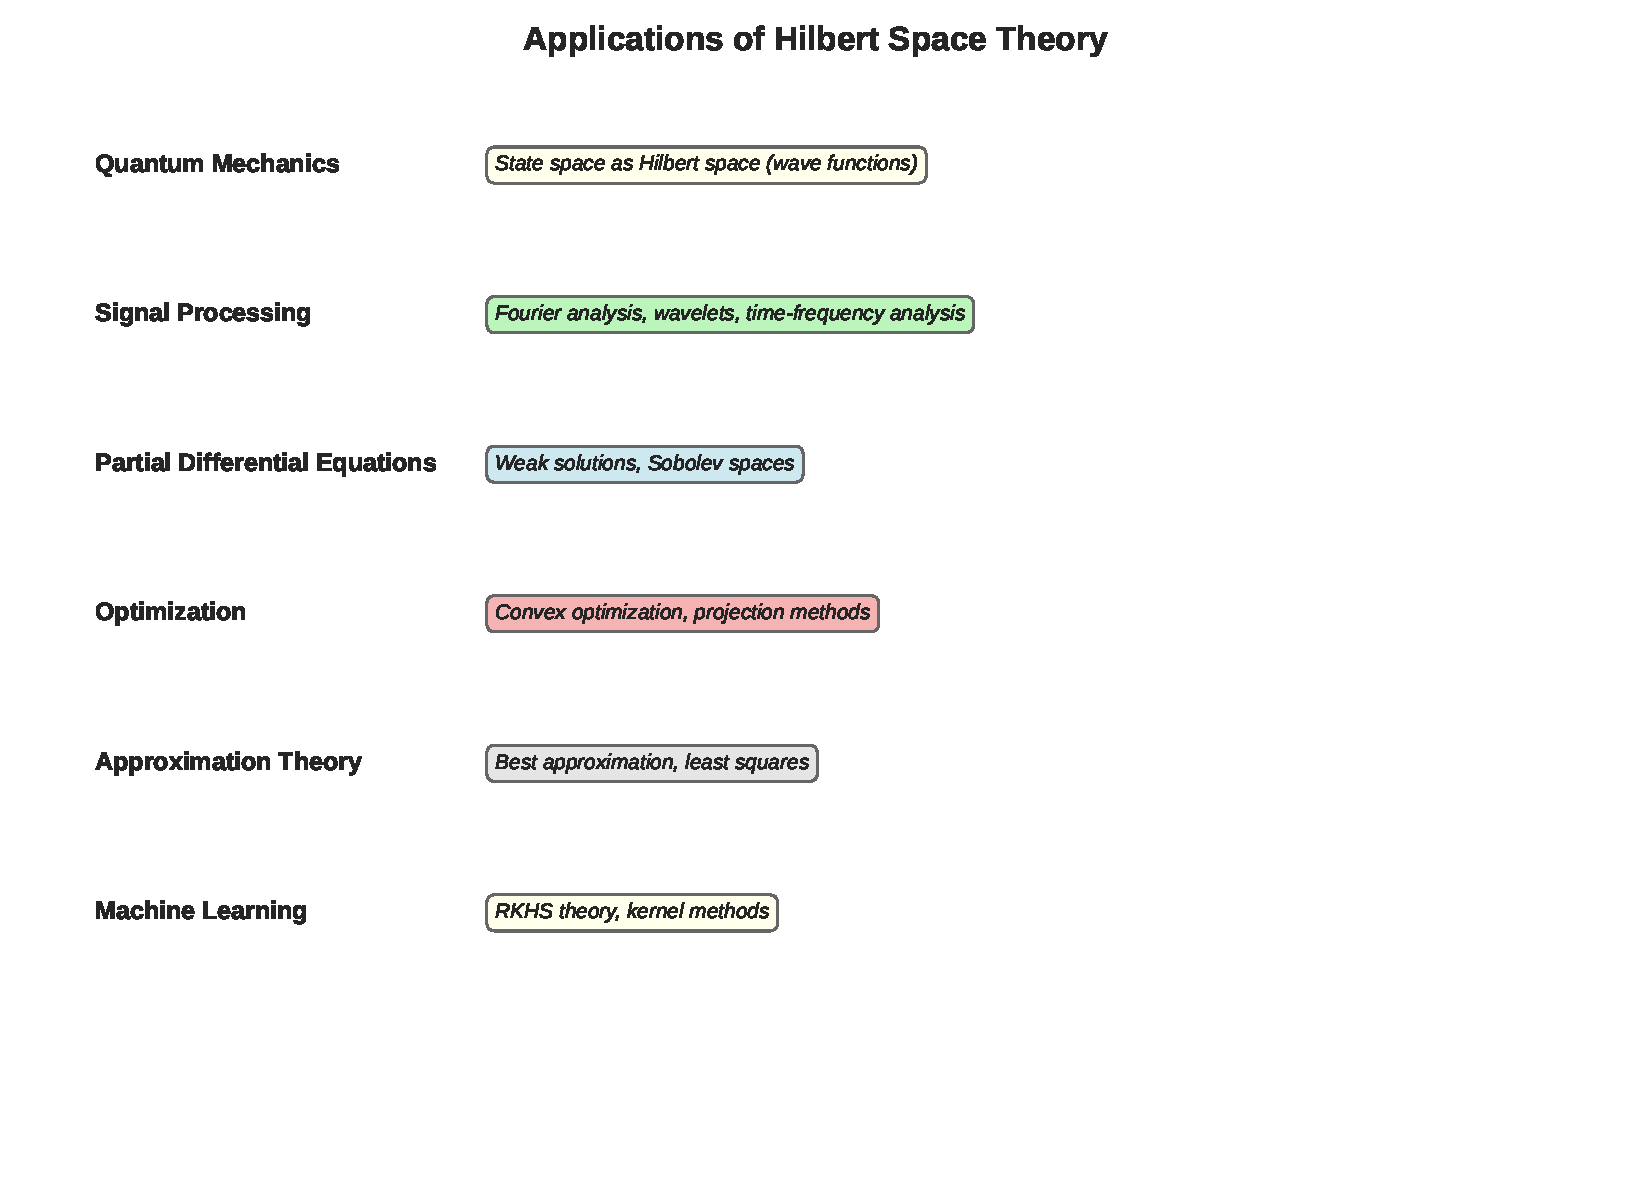
\includegraphics[width=\textwidth]{fig_applications.pdf}

\vspace{0.3cm}

These applications demonstrate the power and universality of Hilbert space theory in mathematics, physics, and engineering.
\end{frame}

\begin{frame}
\frametitle{Induced Norm from Inner Product}

\vspace{-0.3cm}

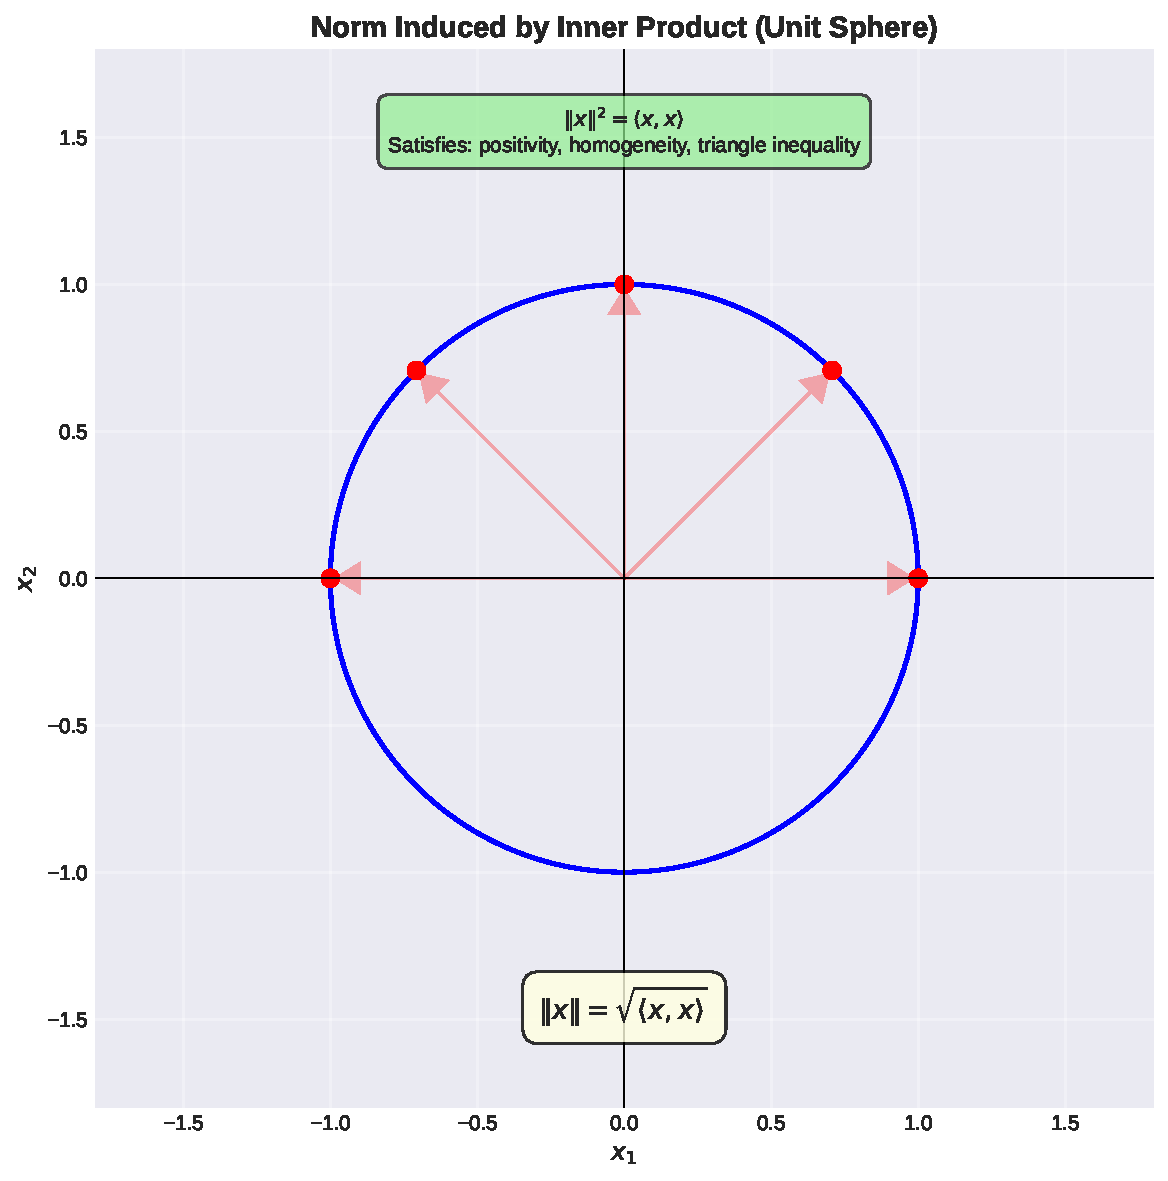
\includegraphics[width=0.8\textwidth]{fig_unit_sphere.pdf}

\vspace{-0.2cm}

The norm $\|x\| = \sqrt{\langle x, x \rangle}$ is the unique norm consistent with the inner product and satisfying the parallelogram law.
\end{frame}

\begin{frame}
\frametitle{Summary: Key Concepts}

\textbf{Inner Product Spaces:}
\begin{itemize}
\item Definition via four properties (positivity, definiteness, conjugate symmetry, linearity)
\item Cauchy-Schwarz inequality: $|\langle x, y \rangle| \leq \|x\|\|y\|$
\item Parallelogram law characterizes inner product structure
\end{itemize}

\vspace{0.2cm}

\textbf{Hilbert Spaces:}
\begin{itemize}
\item Complete inner product spaces
\item Self-dual (dual space isomorphic to itself via Riesz theorem)
\item Examples: $\mathbb{R}^n$, $\ell^2$, $L^2[a,b]$
\end{itemize}

\vspace{0.2cm}

\textbf{Orthogonal Structures:}
\begin{itemize}
\item Orthonormal bases exist (Gram-Schmidt process)
\item Fourier expansions via complete orthonormal systems
\item Parseval's equality relates norms to coefficient sequences
\end{itemize}

\vspace{0.2cm}

\textbf{Convergence:}
\begin{itemize}
\item Strong convergence: $\|x_n - x\| \to 0$
\item Weak convergence: $\langle x_n, y \rangle \to \langle x, y \rangle$ for all $y$
\item Weak compactness of closed balls (Eberlein-Smulian)
\end{itemize}

\vspace{0.2cm}

\textbf{Applications:} Quantum mechanics, signal processing, PDEs, optimization, approximation theory.
\end{frame}

\begin{frame}
\frametitle{References and Further Reading}

\begin{thebibliography}{99}
\bibitem{pathak2018}
Pathak, H.K. (2018). \textit{An Introduction to Nonlinear Analysis and Fixed Point Theory}. Springer.

\bibitem{rudin1976}
Rudin, W. (1976). \textit{Principles of Mathematical Analysis}. McGraw-Hill.

\bibitem{kreyszig1978}
Kreyszig, E. (1978). \textit{Introductory Functional Analysis with Applications}. Wiley.

\bibitem{conway1990}
Conway, J.B. (1990). \textit{A Course in Functional Analysis}. Springer.

\bibitem{brezis2011}
Brézis, H. (2011). \textit{Functional Analysis, Sobolev Spaces and Partial Differential Equations}. Springer.

\bibitem{reed1980}
Reed, M. and Simon, B. (1980). \textit{Methods of Modern Mathematical Physics I: Functional Analysis}. Academic Press.
\end{thebibliography}
\end{frame}

\end{document}
